\documentclass[11pt]{article}
\usepackage[top=1.5cm,bottom=1.5cm,left=1.5cm,right= 1.5cm]{geometry}
%\geometry{landscape}                % Activate for for rotated page geometry
\usepackage[parfill]{parskip}    % Activate to begin paragraphs with an empty line rather than an indent
\usepackage{graphicx}
\usepackage{amssymb}
\usepackage{epstopdf}
\usepackage{setspace}            
\usepackage{amsmath}            
\usepackage{multirow}    
\usepackage{changepage}
\usepackage{lscape}
\usepackage{ulem}
\usepackage{multicol}
\usepackage{dashrule}
\usepackage[usenames,dvipsnames]{color}       
\usepackage{enumerate}
\newcommand{\urlwofont}[1]{\urlstyle{same}\url{#1}}
\newcommand{\degree}{\ensuremath{^\circ}}

\DeclareGraphicsRule{.tif}{png}{.png}{`convert #1 `dirname #1`/`basename #1 .tif`.png}

\newenvironment{choices}{
\begin{enumerate}[(a)]
}{\end{enumerate}}

\pagestyle{empty}

%\newcommand{\soln}[1]{\textcolor{MidnightBlue}{\textit{#1}}}	% delete #1 to get rid of solutions for handouts
\newcommand{\soln}[1]{ \vspace{2.7cm} }

\newcommand{\solnMult}[1]{\textbf{\textcolor{MidnightBlue}{\textit{#1}}}}	% uncomment for solutions
%\newcommand{\solnMult}[1]{ #1 }	% uncomment for handouts

%\newcommand{\pts}[1]{ \textbf{{\footnotesize \textcolor{black}{(#1)}}} }	% uncomment for handouts
\newcommand{\pts}[1]{ \textbf{{\footnotesize \textcolor{red}{(#1)}}} }	% uncomment for handouts

\newcommand{\note}[1]{ \textbf{\textcolor{red}{[#1]}} }	% uncomment for handouts

\definecolor{oiG}{rgb}{.298,.447,.114}
\definecolor{oiB}{rgb}{.337,.608,.741}

\usepackage[colorlinks=false,pdfborder={0 0 0},urlcolor= oiG,colorlinks=true,linkcolor= oiG, citecolor= oiG,backref=true]{hyperref}

%\usepackage{draftwatermark}
%\SetWatermarkScale{4}

\usepackage{titlesec}
\titleformat{\section}
{\color{oiB}\normalfont\Large\bfseries}
{\color{oiB}\thesection}{1em}{}
\titleformat{\subsection}
{\color{oiB}\normalfont}
{\color{oiB}\thesubsection}{1em}{}

\newcommand{\ttl}[1]{ \textsc{{\LARGE \textbf{{\color{oiB} #1} } }}}

\newcommand{\tl}[1]{ \textsc{{\large \textbf{{\color{oiB} #1} } }}}

\begin{document}

Dr. \c{C}etinkaya-Rundel \hfill Data Analysis and Statistical Inference \\

\ttl{Application exercise: \\
3.3 Sample size} 

\section*{GPA at Duke - revisited}

In 2001 the average GPA of students at Duke University was 3.37. This semester we surveyed you, and 63 students responded to the question on GPA. The mean was 3.58, and the standard deviation 0.53. A histogram of the data is shown below.

\begin{center}
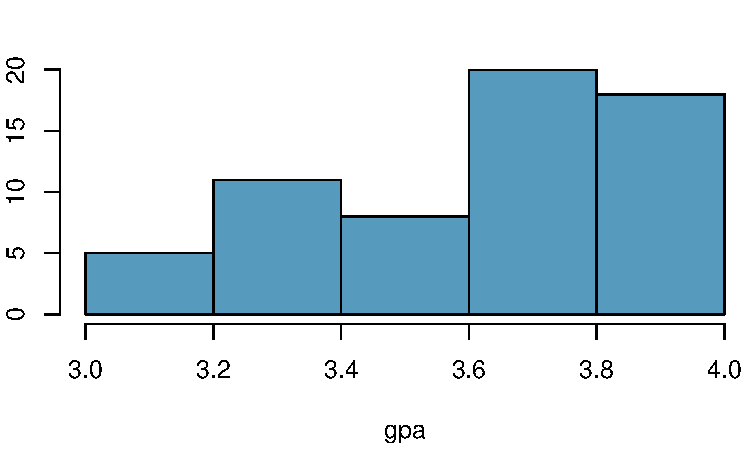
\includegraphics[width=0.5\textwidth]{survey/hist_gpa}
\end{center}

\begin{enumerate}

\item Construct a 95\% confidence interval for the average GPA of all Duke students.

\item If we wanted to cut the margin of error in half while keeping the confidence level the same, how many Duke students would we need to sample?

\item If we wanted to cut the margin of error in half (compared to the original confidence interval from Question 1 above) and increase the confidence level to 98\%, how many Duke students would we need to sample?

\end{enumerate}

%

\end{document}